\documentclass[14pt, oneside]{altsu-report}

\title{Отчет по производствено-эксплуатационной практике}
\author{Д.\,В.~Осипенко}
\groupnumber{595}
\GradebookNumber{}
\supervisor{И.\,А.~Шмаков}
\supervisordegree{ст. преп. каф. ВТиЭ.}
\ministry{Министерство науки и высшего образования}
\country{Российской Федерации}
\fulluniversityname{ФГБОУ ВО Алтайский государственный университет}
\institute{Институт цифровых технологий, электроники и физики}
\department{Кафедра вычислительной техники и электроники}
\departmentchief{В.\,В.~Пашнев}
\departmentchiefdegree{к.ф.-м.н., доцент}
\shortdepartment{ВТиЭ}
% \abstractRU{Большой текст на русском!}
% \abstractEN{Большой текст на английском!}
% \keysRU{компьютерное моделирование, cистема управления версиями}
% \keysEN{computer simulation, distributed version control}

\date{\the\year}

% Подключение файлов с библиотекой.
\addbibresource{graduate-students.bib}

\begin{document}
\maketitle

\setcounter{page}{2}
% \makeabstract
\tableofcontents

\chapter*{Введение}
\addcontentsline{toc}{chapter}{Введение}
Осуществлено прохождение производственно-эксплуатационной практике (далее - практика) направленния подготовки <<Информатика и вычислительная техника>> на базе кафедры Вычислительной техники и электроники (ВТиЭ) Алтайского государственного университета (АлтГУ).  
Периуд прохождения практики 4 недели: с 16 мая, по 11 июня 2022 года. за этот периуд мной произведено:
\begin{enumerate}
  \item Ознакомление с номативно-правовой базой, регламентирующей деятельность программиста на месте практики:
  \begin{enumerate}
    \item Должностная инструкция программиста
    \item Инструкция по охране труда для программиста
    \item Вводный инструктаж
    \item Инструктаж по технике безопасности
  \end{enumerate}
  \item Диагнотика компьтеров на работоспособность, выявление технических проблем.
  \item Установка и настройка программного обеспечения для операционных систем Windows XP, 10 и Linux Ubuntu.
  \item Разработка скриптов для bash и powershell
  \item Разработка мобильного приложения на тему <<Устные вычисления>>
  \item Руководство группой людей
\end{enumerate} 

\subsection*{Цель практики}
\begin{enumerate}
  \item Получить знания и навыки их практического применения в сфере системного администрирования и программирования
  \item Ознакомится со спецификой деятельности системного администратора
  \item Развитие лидерских качеств
\end{enumerate}

\subsection*{Задачи практики}
\begin{enumerate}
  \item  Поиск и изучение руководств по инсталляции, настройке, наладке, использованию программно-аппаратного обеспечения вычислительной техники, информационных и автоматизированных систем;
  \item  Освоение методик использования необходимого программного обеспечения;
  \item  Проверка работоспособности типовых узлов и устройств;
  \item  Использование программного обеспечения для решения практических задач, составление схем приема-передачи данных.
\end{enumerate}



\chapter{Глава. Обязоности и деятельность производимые на предприятии}
\section{Диагностика компьютеров. Устранение найденныйх проблем.}
Диагностика компьютера направленна на выявление проблем в его работе. В нашем случае план тестирования следующий:
\begin{enumerate}
  \item Попытка запуска
  \item Проверка подключенных устройств в BIOS
  \item Проверка настроек BIOS
  \item Проверка работоспособности RAM с помощью программы Memory Test 86 (memtest86) с загрузочной флешки
  \item Проверка HDD на наличие битых секторов с помощью * с загрузочной флешки
\end{enumerate}

В общем случае работа была проведена с 10тью компьютерами, которые в последующем были установленны в 206 аудиторию:

\begin{itemize}
  \item Для двух ПК была произведена замена/установка блока питанию
  \item У 4 ПК была заменена батарейка BIOS
  \item Для 5 ПК устранена проблема с ошибкой объема памяти для дискетоприемника путем изменения значения в BIOS
  \item У 1 ПК устранена проблема c S.M.A.R.T. (self-monitoring, analysis and reporting technology) при загрузке компьютера путем отключения параметра в BIOS
  \item У 5 ПК установлено верное значение даты и времени
  \item Для каждого компьютера установленны RAM примерно на 1гб (в сумме)
  \item Успешно протестированно 9 ПК на наличие ошибок RAM, 10 на проблем с HDD
  \item У 1 ПК выявленны проблеммы с разъемом оперативной памяти материнской платы
  \item Обнаружены две неисправные плашки оперативной памяти
\end{itemize}

\section{Установка Linux Ubuntu. Установка необходимого и удаление предустановленного/ненужного программного обеспечения}
Необходимо установить Linux на один диск с Windows для запуска с помощью Dual Boot. Логично предположить, что производить установку для каждого ПК по отдельности долго и утомительно, поэтому был выбран один ПК, на нем установленна Linux, произведенна настройка, установка всего необходимого программного обеспечения и после этого дополнительно подключается hdd от другого ПК и производится клонирование данных с помощью программы CloneZila. 

Установка Ubuntu linux производилась с помощью стандартного GUI установщика, добавлены дистрибутивы АлтГУ, осуществленно разбиение свободной части диска на три раздела: загрузка (boot), виртуальная память (swap), домашний раздел (root/home). После завершения установки был отредактирован и запущен bash скрипт для скачивания необходимых программных покетов. 

Для Windows XP была произведенна активация с помощью ключа. 
Установленны недостающие драйвера и необходимы программы в 202, 206, 208, 210 аудиториях.

Для Windows 10 был написан скрипт на языке оболочки PowerShell для отключения некоторых служб, удаление предустановленных программ (Xbox, Cortana, ...), увелечения виртуальной памяти. Скрипт опробован и использован в 208 и 210 аудиториях.

\section{Руководство приставленными студентами и первокусниками}
Со второй недели прохождения практики ко мне были приставленны студенты Колледжа АлтГУ, проходящие практику на базе кафедры ВТиЭ. Мной была осуществлена помощь и обучение в проделывание перечисленных выше действиях, распределение обязанностей и раздача указаний при выполнении некоторых действий, например: установка компьютеров на рабочие места; контроль над первокурсниками.

С четвертой недели к подопечным присоеденились первокурсники, проходящие ознакомительную практику. В отношении их выполнялись надзор над выполнением поставленных задач руководством, помощь в разрешение трудностей, контроль посещаемости.

\chapter{Глава. Индивидуальное задание. Приложение для тренировки устных вычислений}
В качестве индивидуального задания было необходимо написать мобильное приложение для тренировки устных вычисленний. 
Разработку мобильного приложения можно произвести с помощью двух способов:
\begin{enumerate}
  \item Нативная разработка
  \item Кроссплатформенная разработка
\end{enumerate}
\section*{Нативная разработка}
Нативная разработка делится на основе двух платформ: Android с языком Kotlin/Java и IOS на Swift/Object-c.

К достоинтсвам данного подхода можно отнести возможность написание нативного кода для каждой операционной системы, что позволяет иметь значительное преймущество в производительности и потенциальной оптимизированности кода. Так же к преймуществам можно отнести добротную документацию и поддержку со стараны вендоров: Google и Apple.

К недостаткам данного способа относятся скорость разработки и невозможность использовать одну кодовую базу для двух видов ОС, что при желании выйти на два рынка может возникнуть необходимость писать одно и тоже приложения для каждой платформы, что выливается в дополнительные затраты на разработку, тестирование.

Данный метод наиболее подходит для приложений, требующих производить множество вычисленний и возможному прямому доступу к возможностям платформы. Примеры таких приложений: Игры, нативные приложения (основанные на функционале платформы).

\section*{Кроссплатформенная разработка}
Лидерами кроссплатформенного рынка являются React Nativ - расширение популярного web-based framework, разработаного компанией Facebook (запрещенной на территории Российской Федерации), призванного использовать написанный раннее код для web-приложения на мобилке. Главным преймуществом является я.п. JavaScript и ОГРОМНОЕ количество frontend-разработчиков, разного уровня, освоивших данный framework. К недостаткам относится малая производительность скомпилированного приложения. 

Другим вариантом, стремительно набирающем популярность является Flutter Framework, разработанный компанией Google, направленный для создание приложений на мобильных устройствах(IOS, Android), ПК(Linux, Windows) и веб страниц с использованием одной базы кода. Отличается относительно высокой производительностью, схожем способом постраения UI с React, быстрорастущим количеством сторонних библиотек и сообщества. Недостатками можно назвать саму компанию Google, которая своеобразно относится к своим проектам (может спокойно тянуть неудачные и не востребованные проекты, забить на потенциально интересные и успешние идеи и пустить все на "свалку проектог гугл") и сложность в отделение бизнес логики от кода ui.

В итоге мной выбор пал в сторону Flutter из-за высокой производительности (по сравнению с React nativ) и желанием в будущем выпустить приложение на Android и IOS.
\section{Проектирование}
Процесс разработки я начал с проектирования приложения. Первым делом я сделал наброски приложения, чтобы определится с функционалом и внешним видом\\
\begin{center}
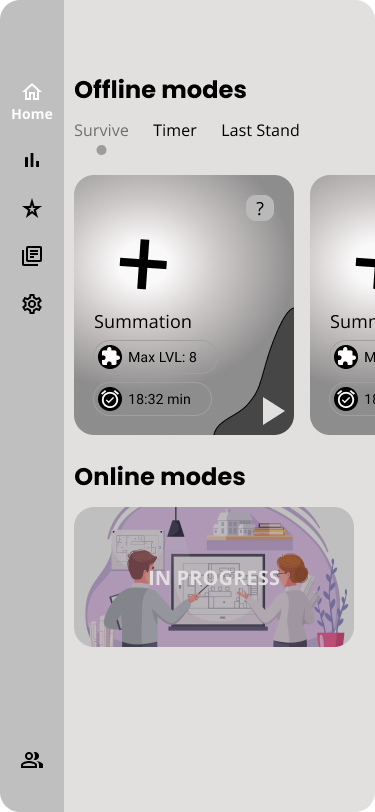
\includegraphics[width=220pt]{home.png}
\hspace{10pt}
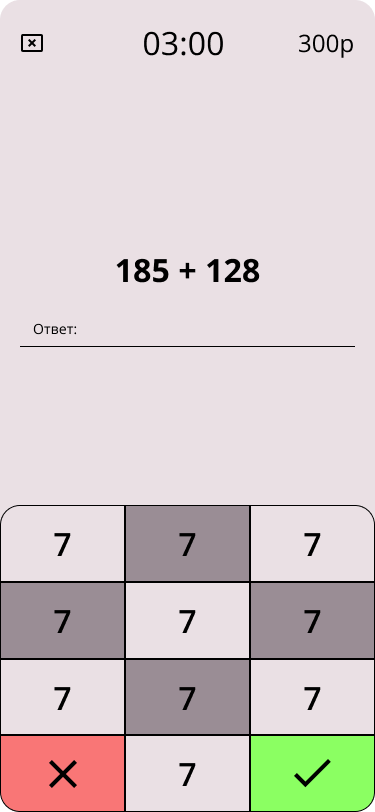
\includegraphics[width=220pt]{game.png}

   Рис 1. Экраны домашней страницы и процесса игры
\end{center}


Далее было решено использовать библиотеку контроля состояний Riverpod, для последующий реализации архитектуры MVC(P) (model view controller (provider)) для отделения бизнес логики от графического интерфейса, но из-за возникших трудностей с dependency injection (передача состояния и значений через дочерние (вложенные) элементы(виджеты)) и трудности создание новых объектов provider при переходе к игровму экрану, основанные на глобальном состоянии providers, окончательный выбор был сделан на библиотеку BLoC, использующие принцыпы bloc, cubit, state(состояние), event(событие)

\begin{center}

\includegraphics[width=\linewidth]{cubit_architecture_full.png}\\
\vspace{20pt}

\includegraphics[width=\linewidth]{bloc_architecture_full.png}\\
   
Рис. 2 Пример BLoC архитектуры с использованием bloc и cubit
\end{center}

\section{Реализация}
Проект представляет из себя 2 экрана: домашний и игровой. Так же имеется вложенный экран для домашнего экрана, необходимы для выбора режима игры.
Для каждого экрана осуществленно извлечение бизнес логики путем использования Bloc элементов, состояний и событий.

\newpage
\begin{center}
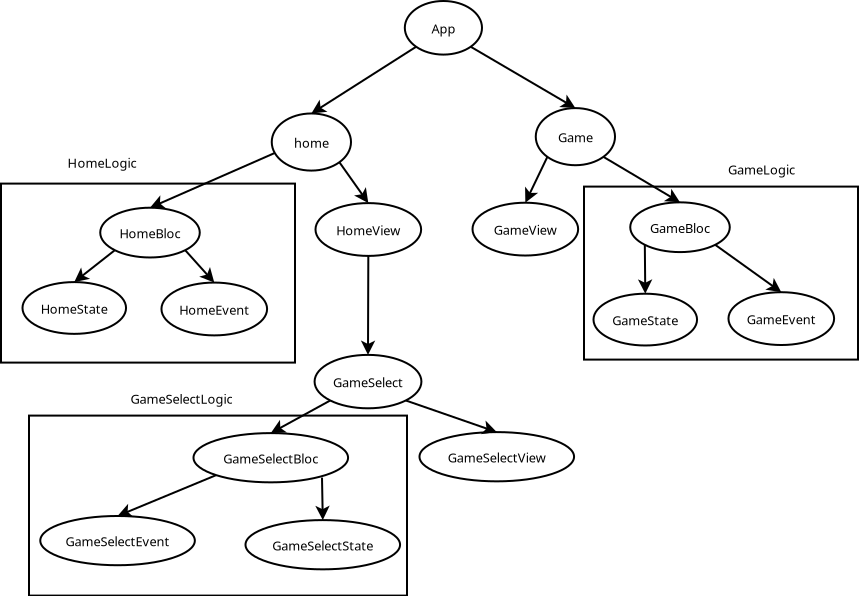
\includegraphics[width=\linewidth]{Struct.png}\\
   
Рис. 3 Структура проекта. 
\end{center}

\chapter*{Заключение}
\addcontentsline{toc}{chapter}{Заключение}

\begin{enumerate}
\item Пример ссылки на литературу~\cite{wikiRUBitbucket}.
\item Пример ссылки на литературу~\cite{wikiRUIdSoftware}.
\item Пример ссылки на литературу~\cite{wikiRUGitHub}.
\end{enumerate}

\newpage
\addcontentsline{toc}{chapter}{Список использованной литературы}
\printbibliography[title={Список использованной литературы}]

\newpage
\chapter*{Приложение B}
\addcontentsline{toc}{chapter}{Приложение B}

\begin{code}
\captionof{listing}{Код приложения}
\label{code:pi-example}
\inputminted[mathescape,linenos,frame=lines,breaklines]{Dart}{src/app/main.dart}

\inputminted[mathescape,linenos,frame=lines,breaklines]{Dart}{src/app/home/home.dart}
\inputminted[mathescape,linenos,frame=lines,breaklines]{Dart}{src/app/home/homeview.dart}
\inputminted[mathescape,linenos,frame=lines,breaklines]{Dart}{src/app/home/homebloc.dart}
\inputminted[mathescape,linenos,frame=lines,breaklines]{Dart}{src/app/home/homestate.dart}
\inputminted[mathescape,linenos,frame=lines,breaklines]{Dart}{src/app/home/homeevent.dart}

\inputminted[mathescape,linenos,frame=lines,breaklines]{Dart}{src/app/gameselect/gameselect.dart}
\inputminted[mathescape,linenos,frame=lines,breaklines]{Dart}{src/app/gameselect/gameselectbloc.dart}
\inputminted[mathescape,linenos,frame=lines,breaklines]{Dart}{src/app/gameselect/gameselectstate.dart}
\inputminted[mathescape,linenos,frame=lines,breaklines]{Dart}{src/app/gameselect/gameselectview.dart}

\inputminted[mathescape,linenos,frame=lines,breaklines]{Dart}{src/app/game/game.dart}
\inputminted[mathescape,linenos,frame=lines,breaklines]{Dart}{src/app/game/gameview.dart}
\inputminted[mathescape,linenos,frame=lines,breaklines]{Dart}{src/app/game/gamebloc.dart}
\inputminted[mathescape,linenos,frame=lines,breaklines]{Dart}{src/app/game/gamestate.dart}
\inputminted[mathescape,linenos,frame=lines,breaklines]{Dart}{src/app/game/gameevent.dart}
\end{code}

\end{document}

